\documentclass{article}

\usepackage{graphicx}
\usepackage{amsmath,amsfonts,amssymb}
\usepackage[colorlinks,bookmarks,bookmarksnumbered,allcolors=blue]{hyperref}
\usepackage[capitalise]{cleveref}
\usepackage[top=0.75in]{geometry}
\usepackage[dvipsnames]{xcolor}
\usepackage{amsmath} 
\usepackage{esvect}
\usepackage{hyperref}
\usepackage{graphicx}
\usepackage{subcaption}
\usepackage{stfloats}

\begin{document}

\author{Joe Spencer}
\title{Airfoil Analysis}
\date{September 18, 2022}
\maketitle

\subsubsection*{Methods}

An airfoil redirects the air flowing past it to generate lift force. When it does this, its motion in the direction of the airstream is resisted by drag force. Lift force and drag force are controlled by the lift and drag equations, shown in Equation 1:

\begin{equation} \label{eq:1}
\begin{aligned}
        	L = \frac{1}{2} \rho u^{2} c_{L} \\
        	D = \frac{1}{2} \rho u^{2} c_{D}
\end{aligned}
\end{equation}
	
Lift and drag force are both proportional to the square of velocity, but they are subjected to different coefficients, the \hyperlink{CL}{Lift Coefficient} and the \hyperlink{CD}{Drag Coefficient}. These coefficients change depending on the \hyperlink{Re}{Reynolds Number} of the wing and its \hyperlink{alpha}{Angle of Attack}, also denoted by the greek letter $\alpha$. In addition to affecting the lift and drag experienced by an airfoil, the angle of attack can also affect its \hyperlink{CM}{Coefficient of Moment}.\newline

This project sought to identify how adjusting an airfoil's \hyperlink{c}{Chord}, or $c$, and \hyperlink{Camber}{Camber} can affect its performance, making it better suited for different environments. For this project, the coordinates of a variety of different airfoils were downloaded from the \href{https://m-selig.ae.illinois.edu/ads.html}{UIUC Applied Aeronautics Group} and then imported them to a Julia program to calculate their \hyperlink{CL}{Lift Coefficient}, \hyperlink{CD}{Drag Coefficient}, \hyperlink{DP}{Pressure Drag Coefficient}, and \hyperlink{CM}{Moment Coefficient}. As can be seen from the included figures, these coefficients each changed with different angles of attack.\newline

For this code, it also became necessary to create similar airfoils, only adjusted slightly for the size and position of their \hyperlink{Camber}{Camber}, and the maximum thickness as a percentage of the \hyperlink{c}{Chord}. To do this, a function was created in the previously mentioned \href{https://github.com/JoeSpencer1/497R-Projects/blob/Airfoil-Analysis/Airfoil_Functions.jl}{header file} to calculate the shape of an airfoil based on its \hyperlink{NACA}{NACA} (National Advisory Committee for Aeronautics) airfoil number. Although there are also other ways to describe an airfoil's profile, this seemed like a clear and efficient method.\newline

Each of the digits in a \hyperlink{NACA}{NACA Airfoil} has its own purpose in defining an airfoil. The first digit is the ratio of the maximum \hyperlink{Camber}{Camber} to the \hyperlink{c}{Chord}, multiplied by ten. The second digit is the distance of the location of maximum camber from the leading edge of the wing, in tenths of the entire length of the wing. The third and fourth digit define the maxim wing thickness as a percentage of the Chord. The profiles of both the top and bottom of the wing can be described by Equations 2 and 3. In these Equations, $x$ represents the distance from the front of the wing, $y_{t}$ represents the wing thickness at $x$, $y_{c}$ represents the location of the wing's center at $x$, $t$ represents the maximum thickness as a decimal percentage of the \hyperlink{c}{chord}, $m$ denotes the wing's maximum camber as a percent of the wing's cord length, and $p$ is the distance of the maximum camber from the front of the wing, in tenths.

\begin{equation} \label{eq:2}
\begin{aligned}
	y_{c} = \frac{m}{p^2} (2 p x - x^2) \qquad \qquad \qquad 0 \leq x \leq p \\
	y_{c} = \frac{m}{(1 - p)^2} ((1 - 2 p) + 2 p x - x^2) \qquad \qquad \qquad p \leq x \leq 1
\end{aligned}
\end{equation}

\begin{equation} \label{eq:3}
\begin{aligned}
	y_{t} = 5 t [ 0.2969 \sqrt{x} - 0.1260 x - 0.3516 x^{2} + 0.2843 x^{3} - 0.1015 x^{4}]
\end{aligned}
\end{equation}

The \href{https://docs.juliahub.com/Xfoil/Mlbda/0.4.0/}{Xfoil.jl} Julia wrapper, a potential-flow code, was employed to calculate the coefficients of lift, drag, and moment. A \hyperlink{PFC}{Potential-flow Code} divides the wing into many small plates and calculates the lift, drag, pressure drag, and moment coefficients for each of these points along its length. This program is repeated with different starting estimates for each coefficient until it either converges or is run a set number of times. In the interface that was developed, the user can adjust the limit of how many times the code can run before it stops.\newline

The \href{https://github.com/JoeSpencer1/497R-Projects/blob/Airfoil-Analysis/Airfoil_Analysis.jl}{Julia file} created for this project and its accompanying \href{https://github.com/JoeSpencer1/497R-Projects/blob/Airfoil-Analysis/Airfoil_Functions.jl}{header file} could control separately for different input options. The final function uses a default angle step size of 1 degree, with 20,000 iterations, from maximum and minimum angles chosen by the user.\newline

\subsubsection*{Results and Discussion}

This research found that adjusting the Reynolds number, angle of attack, thickness, and camber amount and position all affect the forces experienced by an airfoil. These forces are described by Equation \ref{eq:1} on the first page. Figure \ref{fig:1} and Figure \ref{fig:2} show that airfoils with a larger \hyperlink{c}{Camber} experience more lift force. The airfoils shown in Figure \ref{fig:1} and Figure \ref{fig:2} experience the same increase in \hyperlink{CD}{Drag Coefficient} as they increase their Camber-to-Cord ratio. Both coefficients increased with increasing angle of attack. On the range from -8$^{\circ}$ to 8$^{\circ}$ shown in the graphs, the Drag Coefficient increased as angle of attack became either more positive or more negative.\newline

Table 1 contains a list of all the airfoil NACA numbers and Reynolds numbers used in this lab. Clicking on the \color{blue}hyperlink number \color{black} below each NACA number will jump to the plot of its lift, drag, or moment coefficients compared to angle of attack. \newline

\begin{table}[bp]
	\centering
	\title{Table 1: Airfoils Modeled by Program \newline}
	\title{\emph{A link to the graph for each airfoil is in its bottom row.}} \label{table:1}
	\begin{tabular}{ | c | c | c | c | c | c | c | c | c | c |}
		\hline
		 \textbf{Profile} & 1310 & 2310 & 3310 & 1412 & 2412 & 3412 & 2209 & 2209 & 2209 \\ \hline
		 \textbf{\emph{Re}} & 100,000 & 100,000 & 100,000 & 100,000 & 100,000 & 100,000 & 100,000 & 200,000 & 300,000 \\ 
		 \textbf{Link} & \ref{fig:1} & \ref{fig:1} & \ref{fig:1} & \ref{fig:2} & \ref{fig:2} & \ref{fig:2} & \ref{fig:3} & \ref{fig:3} & \ref{fig:3} \\ \hline \hline
		 \newline
		 \textbf{Profile} & 1115 & 1115 & 1115 & 2208 & 2213 & 2218 & 2114 & 2214 & 2314 \\ \hline
		 \textbf{\emph{Re}} & 100,000 & 200,000 & 300,000 & 100,000 & 100,000 & 100,000 & 100,000 & 100,000 & 100,000 \\ 
		 \textbf{Link} & \ref{fig:4} & \ref{fig:4} & \ref{fig:4} & \ref{fig:5} & \ref{fig:5} & \ref{fig:5} & \ref{fig:6} & \ref{fig:6} & \ref{fig:6} \\ \hline
	\end{tabular}
\end{table}

\begin{figure}
  \centering
  \subfloat[]{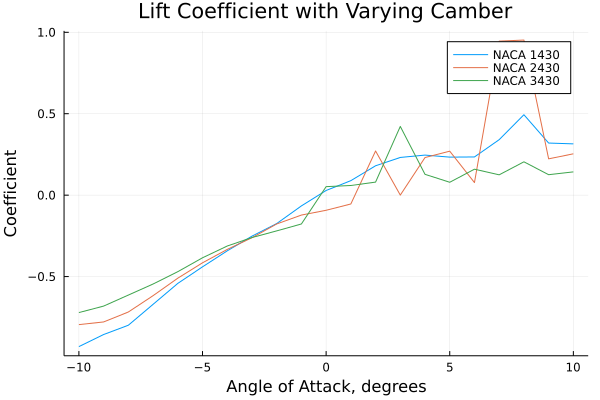
\includegraphics[width=.30\textwidth]{Figure1.png}} \label{fig:1}
  \subfloat[]{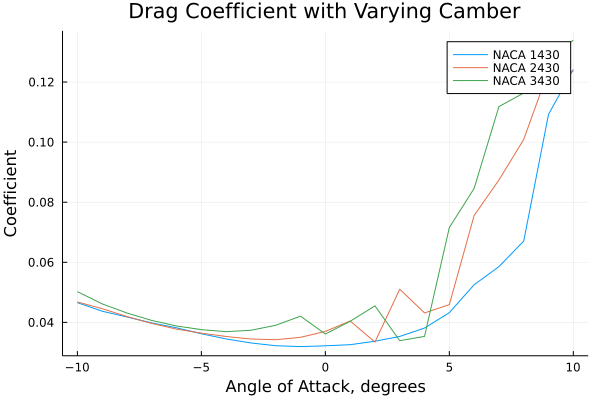
\includegraphics[width=.30\textwidth]{Figure2.png}} \label{fig:1}
  \subfloat[]{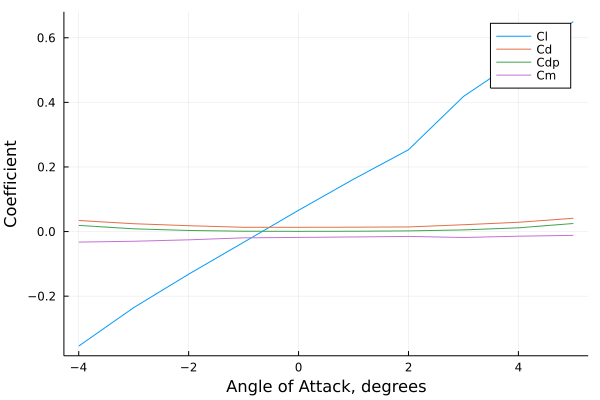
\includegraphics[width=.30\textwidth]{Figure3.png}} \label{fig:1}
  \caption{This figure shows the Lift \textbf{(a)}, Drag \textbf{(b)}, and moment \textbf{(c)} coefficients of airfoils of varying camber length.}
  \label{run5}
\end{figure}

One difficulty that was encountered during the analysis of these airfoils was making smooth graphs for them over their entire angle range. This was difficult because the airfoils compared were sometimes significantly different. For example, Airfoils 1 and 2 had very close \hyperlink{NACA}{NACA Numbers}, with the only difference between them being their first digit. This 1-digit difference meant, though, that Airfoil 2 had twice as much \hyperlink{c}{Camber}. This meant that although their behaviors could be plotted on the same plane in Figures \ref{fig:1}, a, b, and c, they were very different. This made it difficult to plot converging solutions for the different coefficients of these wing types on the same plane.\newline

The plots in Figure \ref{fig:1} and Figure \ref{fig:2} appear to have a similar upward slope, which is expected. As the wing tilts upwards with an increasing angle of attack \hyperref{aplha}{$\alpha$}, its \hyperlink{CL}{Lift Coefficient} increases from negative to positive for both airfoils. A notable difference, though, is that for the airfoils with their maximum camber further forward shown in Figure \ref{fig:1} had a greater drag coefficient at lower angles than those in Figure \ref{fig:2}.

\begin{figure}[!htb]
  \centering
  \subfloat[]{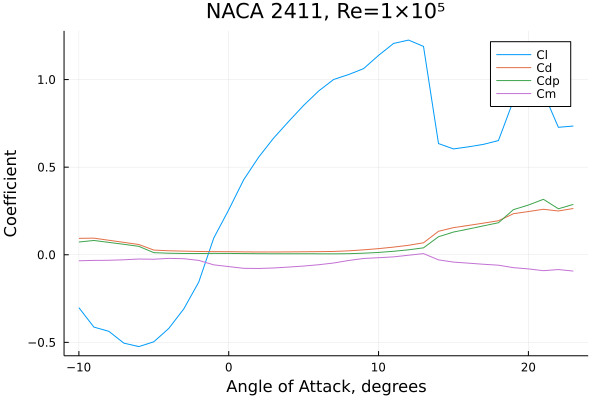
\includegraphics[width=.35\textwidth]{Figure4.png}} \label{fig:2}
  \subfloat[]{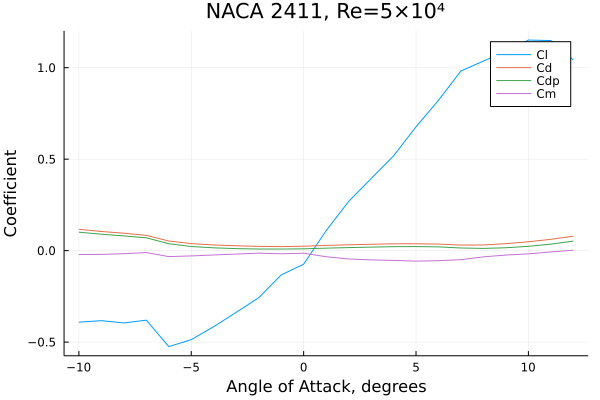
\includegraphics[width=.35\textwidth]{Figure5.png}} \label{fig:2}
  \subfloat[]{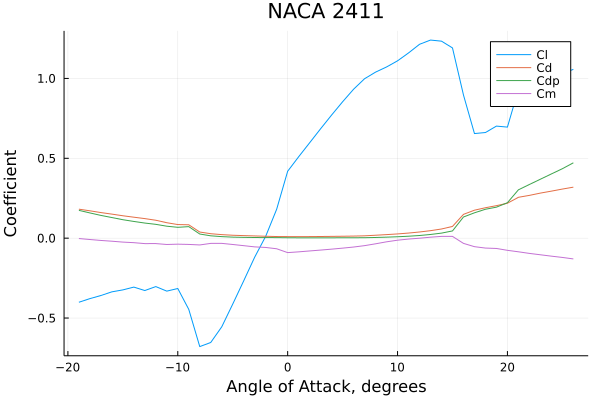
\includegraphics[width=.35\textwidth]{Figure6.png}} \label{fig:2}
  \caption{Figure \textbf{(a)} shows the Lift Coefficients, and Figures \textbf{(b)} and \textbf{(c)} show the Drag and Moment Coefficients for these Airfoils of varying camber length.}
  \label{run5}
\end{figure}

Adjusting the Reynolds Number of an airfoil also changed its behavior significantly. The unit-less Reynolds number of an airfoil, described by Equation 4, can change for an aircraft even as its velocity or the air density changes.

\begin{equation} \label{eq:4}
\begin{aligned}
        	Re = \frac{uL}{\nu} \\
	= \frac{\rho uL}{\mu} 
\end{aligned}
\end{equation}
\newline

\begin{figure}[!htb]
  \centering
  \subfloat[]{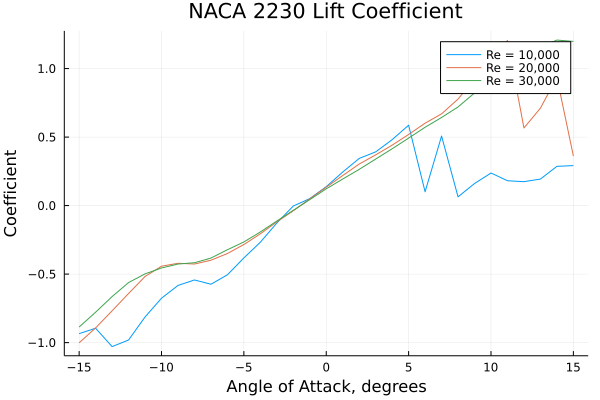
\includegraphics[width=.35\textwidth]{Figure7.png}}
  \subfloat[]{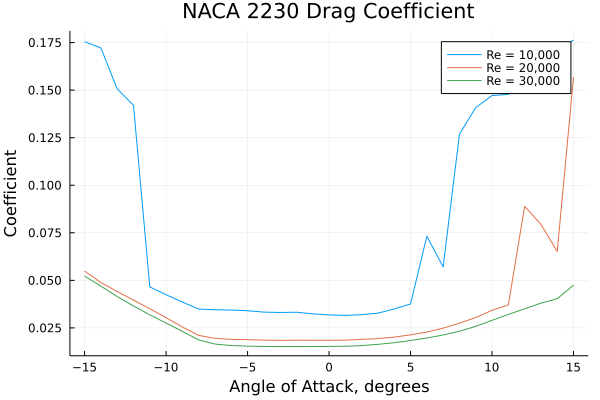
\includegraphics[width=.35\textwidth]{Figure8.png}} 
  \subfloat[]{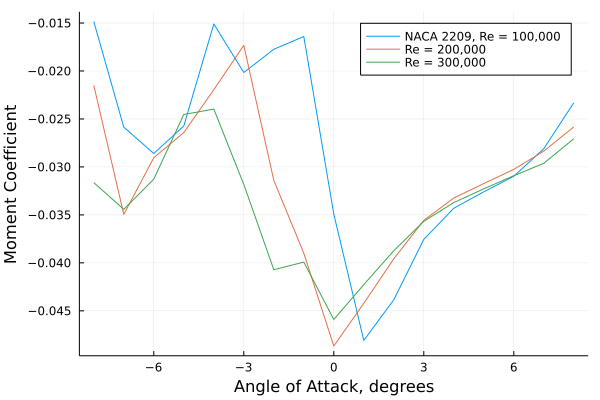
\includegraphics[width=.35\textwidth]{Figure9.png}}
  \caption{Figure \textbf{(a)} shows an Airfoil's Lift Coefficient varied by Reynolds number. Figures \textbf{(b)} and \textbf{(c)} do the same for its Drag and Moment Coefficients.}
  \label{run5}
\end{figure}

Both the NACA 2230 Airfoil shown in Figure \ref{fig:3} and the NACA 1120 Airfoil in Figure \ref{fig:4} appear to increase in \hyperlink{CL}{Lift Coefficient} more rapidly at lower \hyperlink{Re}{Reynolds Numbers}. Their \hyperlink{CD}{Drag Coefficients} appear higher at low Reynolds Numbers in both Figure \ref{fig:3} and Figure \ref{fig:4}. At low Reynolds numbers their \hyperlink{CM}{Moment Coefficients} are both higher, but decrease more quickly.

\begin{figure}[!htb]
\minipage{0.32\textwidth}
  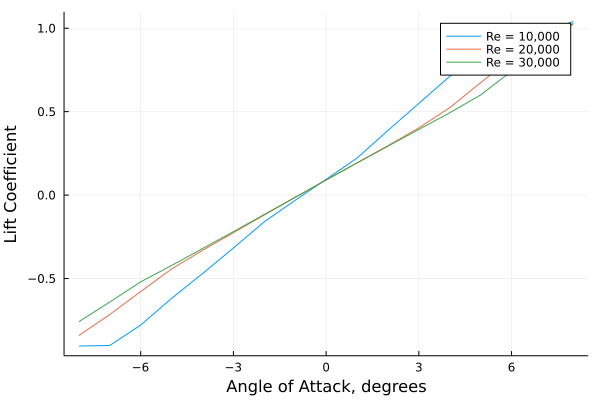
\includegraphics[width=\linewidth]{Figure10.png}
  \caption{NACA 1115 Lift Coefficients Varied by Reynolds Number}\label{fig:10}
\endminipage\hfill
\minipage{0.32\textwidth}
  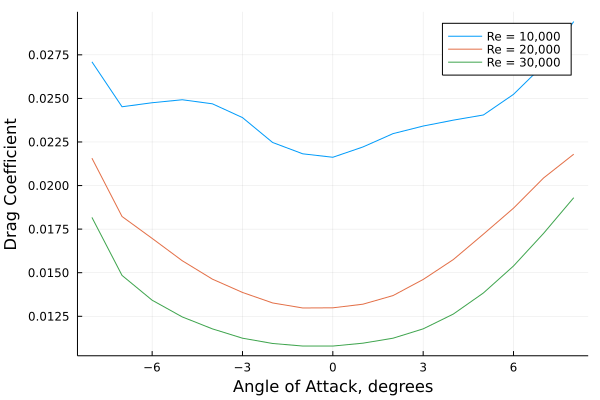
\includegraphics[width=\linewidth]{Figure11.png}
  \caption{NACA 1115 Drag Coefficients Varied by Reynolds Number}\label{fig:11}
\endminipage\hfill
\minipage{0.32\textwidth}
  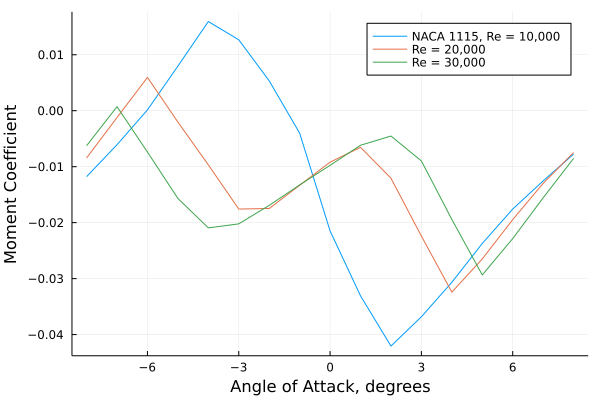
\includegraphics[width=\linewidth]{Figure12.png}
  \caption{NACA 1115 Moment Coefficients Varied by Reynolds Number}\label{fig:12}
\endminipage
\end{figure}

\begin{figure}[!htb]
  \centering
  \subfloat[]{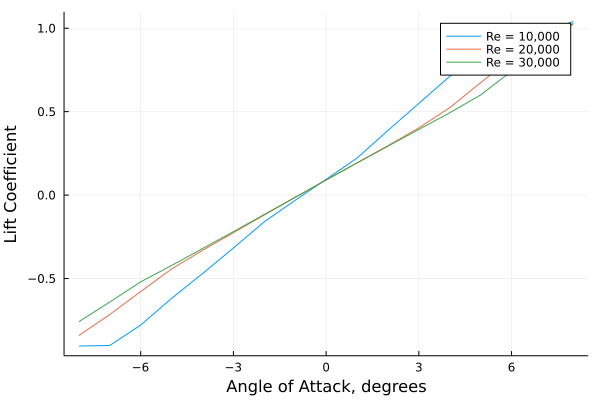
\includegraphics[width=.35\textwidth]{Figure10.png}} 
  \subfloat[]{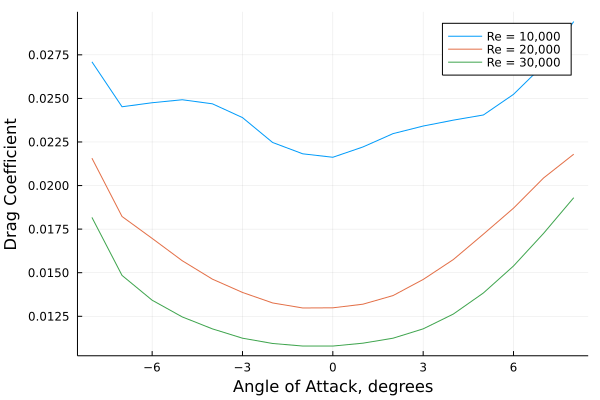
\includegraphics[width=.35\textwidth]{Figure11.png}} 
  \subfloat[]{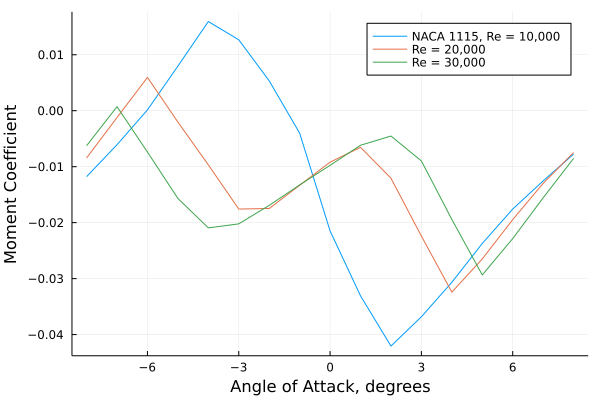
\includegraphics[width=.35\textwidth]{Figure12.png}}
  \caption{The Lift Coefficient of a NACA 1115 airfoil is shown in \textbf{(a)} at varying Reynolds numbers. Its Drag Coefficients are shown in \textbf{(b)} and its Moment Coefficient is shown in \textbf{(c)}}
  \label{run5}
\end{figure}

Figure \ref{fig:5} shows that varying the \hyperlink{Th}{Wing Thickness} only slightly can have huge impacts on the Lift, Drag, and Moment experienced by an airfoil. This is because adjusting a wing's thickness varies the position of its surface at each point along its profile, which add up to flow to be redirected in significantly different ways.

\begin{figure}[!htb]
  \centering
  \subfloat[]{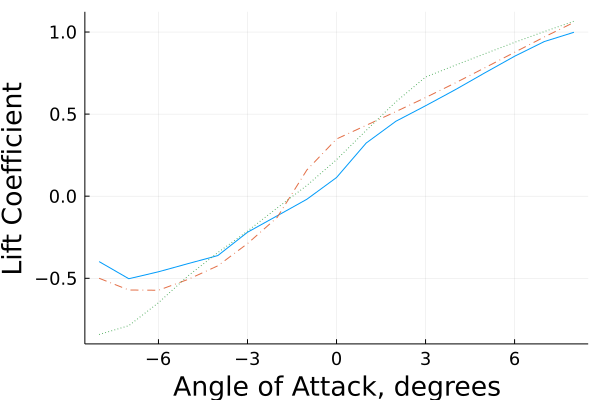
\includegraphics[width=.35\textwidth]{Figure13.png}} 
  \subfloat[]{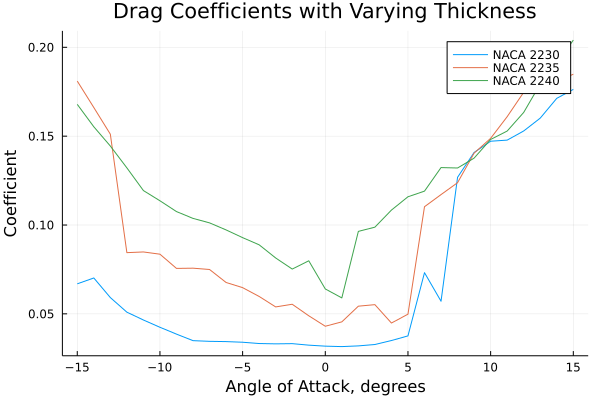
\includegraphics[width=.35\textwidth]{Figure14.png}} 
  \subfloat[]{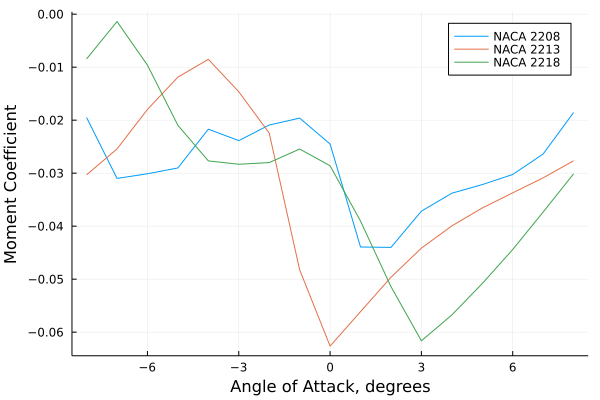
\includegraphics[width=.35\textwidth]{Figure15.png}}
  \caption{Figures \textbf{(a)}, \textbf{(b)}, and \textbf{(c)} show the changes in Lift, Drag, and Moment coefficients that occur when an airfoil's Maximum Camber location is adjusted.}
  \label{run5}
\end{figure}

Although \hyperlink{Th}{Wing Thickness} has been shown to significantly impact an airfoil's Lift, Drag, and Moment Coefficients, Figure \ref{fig:6} shows that the position of the \hyperlink{Camber}{Maximum Camber} does not seem to significantly impact the Lift Coefficient. Figure \ref{fig:6} shows that drag coefficient is hardly not impacted as much either. Moment coefficient is perhaps changed the most, shown in Figure \ref{fig:6}, but this is still much less than the change caused by wing thickness shown in Figure \ref{fig:5}.

\begin{figure}[!htb]
  \centering
  \subfloat[]{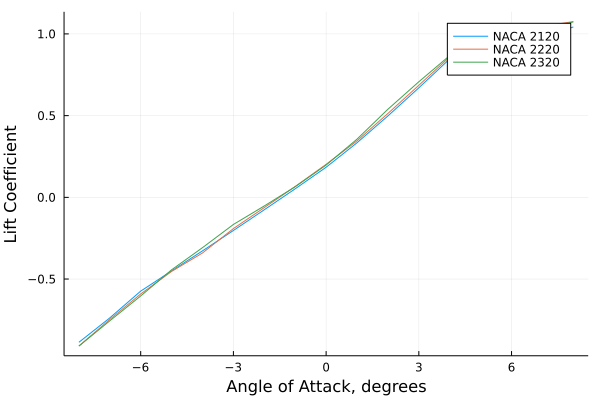
\includegraphics[width=.35\textwidth]{Figure16.png}} 
  \subfloat[]{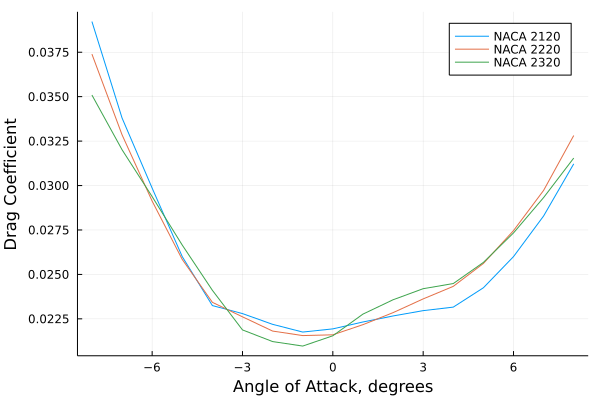
\includegraphics[width=.35\textwidth]{Figure17.png}} 
  \subfloat[]{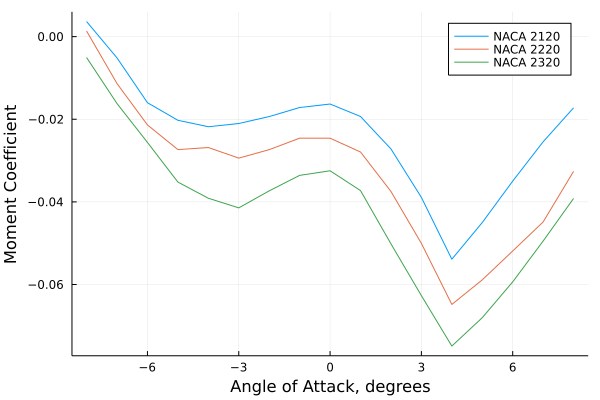
\includegraphics[width=.35\textwidth]{Figure18.png}}
  \caption{Figure \textbf{(a)} displays changes in an airfoil's Lift Coefficient according to Maximum Camber Location. Figure \textbf{(b)} shows what happens to its Drag Coefficient, and changes in the Moment Coefficient can be observed in Figure \textbf{(c)}.}
  \label{run5}
\end{figure}

I found in this airfoil analysis that an airfoil experiences different \hyperlink{CL}{Lift}, \hyperlink{CL}{Drag}, and \hyperlink{CM}{Moment} forces at different \hyperlink{alpha}{Angles of Attack}. I found that in general, Lift force increases with increasing angle of attack, and drag force behaves as a parabola with a minimum near zero. Zooming out further beyond the 16-degree domain of these graphs would show that these coefficients actually behave as sinusoidal waves as the airfoil's angle of attack moves around in a circle.\newline

A surprising finding was that the Lift and Drag coefficients experienced by an airfoil are not significantly impacted by its maximum camber location, as seen in Figure 18. It must not actually impact where airflow is actually redirected. Thicker wings appear to experience greater Drag and lower Lift, as seen in Figures 13. and 14. A higher Reynolds Number appears to correspond to a faster increase in the \hyperlink{CL}{Lift Coefficient}, but also a much higher \hyperlink{CD}{Drag Coefficient}. \newline

For this project, I also completed the example in the \href{https://flow.byu.edu/Xfoil.jl/stable/}{Xfoil.jl Documentation} provided with the lab, using \href{https://github.com/JoeSpencer1/497R-Projects/blob/Airfoil-Analysis/Demo.jl}{this code}.

\clearpage

\section{Glossary}
\begin{itemize}
		
	\item \hypertarget{alpha}{Angle of Attack, $\alpha$} - The angle of attack, $\alpha$ is the angle between the motion of oncoming fluid and the chord line of the wing. a positive $\alpha$ corresponds to a wing tilted upwards.
	
	\item \hypertarget{Camber}{Camber} - The Camber of an airfoil is represented by the Camber Line, which runs halfway between its top and bottom surfaces. This line represents the curvature of an airfoil. An airfoil with positive camber is slightly convex on top and slightly concave on its bottom.
	
	\item \hypertarget{c}{Chord, $c$} - An airfoil's Chord is the imaginary line running straight from the tip of an airfoil to its tail. The chord line is used to find an airfoil's \hyperlink{alpha}{Angle of Attack}.

	\item \hypertarget{CD}{Drag Coefficient (2D), $c_{D}$} - The drag coefficient determines how much drag force opposing motion will be experienced. It comes from a combination of \hyperlink{DP}{Pressure Drag}, also called Form Drag, and \hyperlink{VD}{Viscous Drag} or Skin Friction. The drag force equation describes it in this way: 
		\begin{equation} \label{eq:13}
		\begin{aligned}
        			D = \frac{1}{2} \rho u^{2} c_{D}
	    	\end{aligned}
		\end{equation}
	
	\item \hypertarget{Vinf}{Freestream Velocity, $V_{\infty}$} - The velocity of an oncoming air flow directly upstream from an airfoil, before it interacts with it.
		
	\item \hypertarget{CL}{Lift Coefficient (2D), $c_{L}$} - The lift coefficient is used in the equation below to define how much lift force acts perpendicular to the direction of the oncoming fluid flow.
		\begin{equation} \label{eq:14}
		\begin{aligned}
        			L = \frac{1}{2} \rho u^{2} c_{L}
	    	\end{aligned}
		\end{equation}
	
	\item \hypertarget{LC}{Lift Curve Slope} - The lift curve plots the \hyperlink{CL}{Lift Coefficient} against the \hyperlink{alpha}{Angle of Attack}. This shows the effect that changing the angle of attack will have on the plane's total lift force.
		
	\item \hypertarget{M}{Mach Number, $M$} - The Mach number is the velocity of an object in proportion to the speed of sound in its medium. When an airfoil is traveling near the speed of sound, its top portions can have fluid velocity above Mach 1. When an airfoil is traveling above Mach 1, the fluid on both sides of it also have velocities above mach 1 while there are points directly before and after it that are below Mach 1.
		\begin{equation} \label{eq:15}
		\begin{aligned}
        			M = \frac{u}{c}
	    	\end{aligned}
		\end{equation}
		
	\item \hypertarget{DP}{Pressure Drag} - Pressure Drag, also called Form Drag, comes from the the formation of a vacuum behind an object. The object experiences higher pressure ahead of it than behind it, so the pressure difference pushes it backwards.
		
	\item \hypertarget{CM}{Pitching Moment Coefficient (2D), $c_{M}$} - The moment coefficient is used to calculate the pitching moment a wing will experience from its dynamic pressure $q$, area $S$, and chord length $c$.
		\begin{equation} \label{eq:16}
		\begin{aligned}
        			M = q S e c_{M}
	    	\end{aligned}
		\end{equation}

	\item \hypertarget{AP}{Polar} - The Airfoil Polar is a plot showing the  \hyperlink{CL}{Lift} and  \hyperlink{CD}{Drag} coefficients corresponding with each \hyperlink{alpha}{Angle of Attack} for an airfoil. Examining the ratios of lift to drag is instrumental in choosing the optimal Angle of Attack.
	
	\item \hypertarget{PFC}{Potential-Flow Code} - A potential-flow code calculates the \hyperlink{CL}{lift}, \hyperlink{CD}{drag}, and \hyperlink{CM}{moment} forces an airfoil experiences at many different points along it. Potential-flow theory assumes constant, incompressible, inviscid fluid flow. It calculates the coefficient for each of these small points and then combines them to find the coefficients along the entire wing.
	
	\item \hypertarget{Re}{Reynolds Number, $Re$} - The Reynolds Number is a unit-less number for fluid flow described by the equation below. It can be used to predict patterns in the fluid's flow, using its flow speed $u$, characteristic length $L$, and kinetic viscosity $\nu$, or else by its density $\rho$, flow speed $u$, characteristic length $L$, and fluid density $\mu$.
		\begin{equation} \label{eq:17}
		\begin{aligned}
        			Re = \frac{uL}{\nu} \\
			= \frac{\rho uL}{\mu} 
	    	\end{aligned}
		\end{equation}
	
	\item \hypertarget{ST}{Stall} - Stall occurs when an airfoil's \hyperlink{alpha}{Angle of Attack} is too great in magnitude. When the angle of attack is too great, flow separation occurs, reducing rather than augmenting the airfoil's \hyperlink{CL}{Lift Coefficient} as the Angle of Attack increases.
	
	\item \hypertarget{Th}{Thickness} - An airfoil's thickness can be measured in two different ways, either along its \hyperlink{c}{Chord Line} or along its \hyperlink{Camber}{Camber Line}. Thickness measured perpendicular to the Camber Line is also called the American Convention, and thickness measured perpendicular to the Chord Line is also called the British Convention.
	
	\item \hypertarget{VD}{Viscous Drag} - Viscous Drag, also called Skin Friction, is drag caused by friction with the fluid particles flowing past an airfoil. Along with \hyperlink{PD}{Pressure Drag}, it contributes to an airfoil's total \hyperlink{CD}{Drag Coefficient} airfoil.
		
	\item \hypertarget{NACA}{4-Digit NACA Airfoil} - A wing shape developed by the National Advisory Committee for Aeronautics (NACA). The first digit is the maximum \hyperlink{Camber}{Camber} in tenths of the \hyperlink{c}{Chord}. The second digit is the distance in tenths of the maximum Camber from the leading edge, out of ten. the final two digits are the maximum wing thickness as a percentage of the Chord. Descriptions of other NACA numbers can also be found on this \href{https://en.wikipedia.org/wiki/NACA_airfoil}{Wikipedia Article}. 
	
\end{itemize}

\end{document}